
	\subsubsection{Use-Case Instance - uciugUserActivity:ugUserActivity}
	
	The actor administrator will open the statics the activity of the users,there he can find out how many users are active at any time. Also the abstract user System give the information		  
	\begin{operationmodel}
	\addheading{usergoal Use-Case Instance}
	\adddoublerow{Instantiated Use Case}{ugUserActivity}
	\adddoublerow{Instance ID}{uciugUserActivity}
	
	\end{operationmodel} 

	
	Figure \ref{fig:lu.uni.lassy.excalibur.examples.icrash-RE-UC-uci-uciugUserActivity}
	The administrator click the button to open the statics so the system has to call the information for the number of the user compared with the time and send it back to the Administrator so he can see it. 
	
	\begin{figure}[htbp]
	\begin{center}
	
	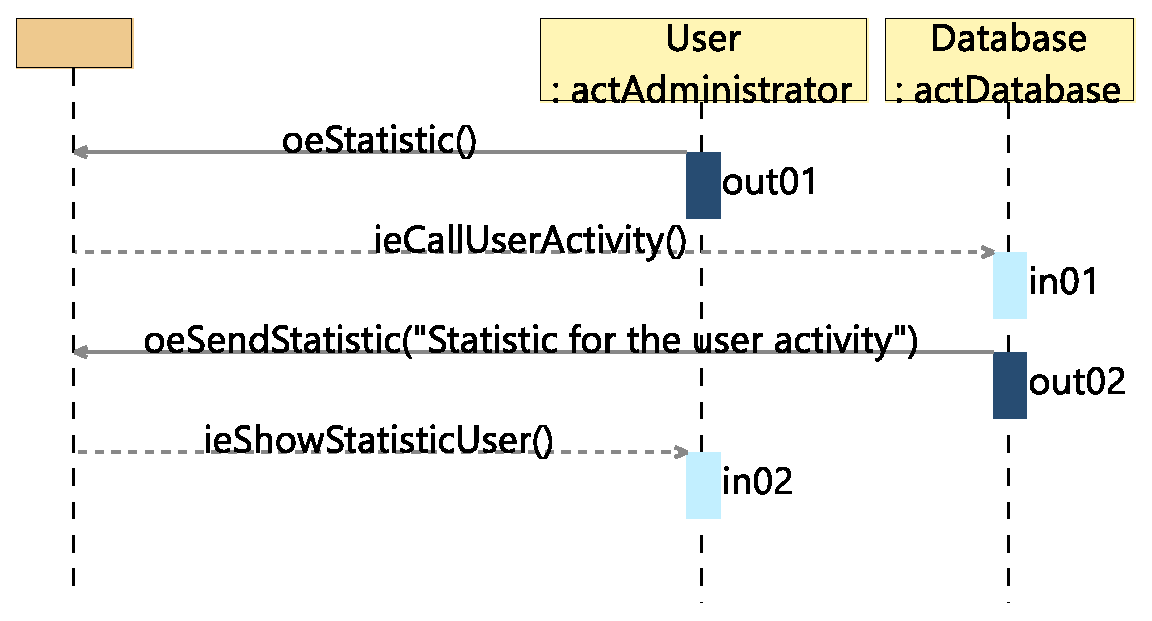
\includegraphics[
	angle=0
	,width=1.0\textwidth
	]{./images-report-gen/usecase-model/usergoal/uci-uciugUserActivity.eps}
	\end{center}
	\caption[lu.uni.lassy.excalibur.examples.icrash Sequence Diagram: uci-uciugUserActivity]{The number of the user compared with the time}
	\label{fig:lu.uni.lassy.excalibur.examples.icrash-RE-UC-uci-uciugUserActivity}
	\end{figure}
	\vspace{0.5cm}
